\documentclass[tikz,margin=6pt]{standalone}
\usepackage{pgfplots}
\pgfplotsset{compat=1.12}

\begin{document}
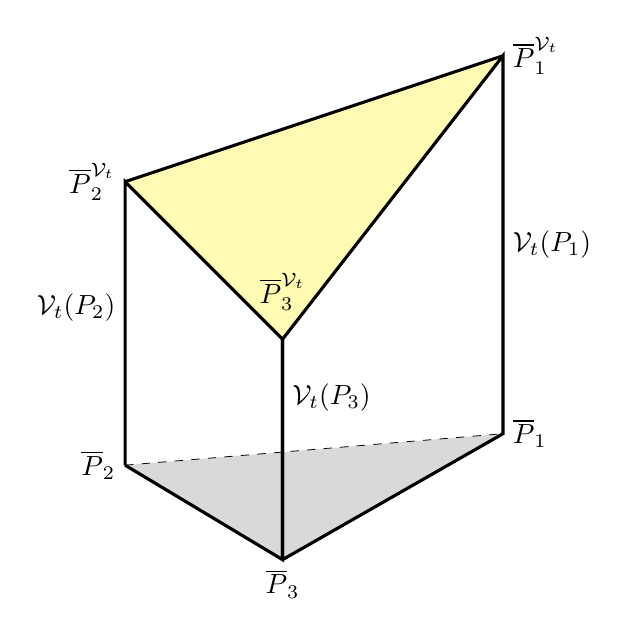
\begin{tikzpicture}[scale=0.8]

\draw[dashed, fill=gray!30, line width=0.1mm] (0,1.5) -- (6,2) -- (2.5,0) -- (0,1.5);
\draw[dashed, fill=yellow!30, line width=0.1mm] (6,8) -- (0,6) -- (2.5,3.5) -- (6,8);
\draw[line width=0.4mm] (0,1.5) -- (0,6) -- (2.5,3.5)  -- (2.5,0) -- (0,1.5);
\draw[line width=0.4mm] (2.5,0) -- (6,2) -- (6,8)  -- (2.5,3.5) -- (2.5,0);
\draw[line width=0.4mm] (6,8) -- (0,6);

\node[anchor=east] at (0,4) {$\mathcal{V}_t(P_2)$};
\node[anchor=east] at (0,1.5) {$\overline{P}_2$};
\node[anchor=south west] at (2.5,2.2) {$\mathcal{V}_t(P_3)$};
\node[anchor=north] at (2.5,0) {$\overline{P}_3$};
\node[anchor=west] at (6,5) {$\mathcal{V}_t(P_1)$};
\node[anchor=west] at (6,2) {$\overline{P}_1$};

\node[anchor=east] at (0,6) {$\overline{P}_2^{\mathcal{V}_t}$};
\node[anchor=west] at (6,8) {$\overline{P}_1^{\mathcal{V}_t}$};
\node[anchor=south] at (2.5,3.8) {$\overline{P}_3^{\mathcal{V}_t}$};


\end{tikzpicture}
\end{document} 